\chapter{Methodology}
\label{methodology}

\section{Project management methodology}
I will use a cyclical, evolutionary method. This will involve:
\begin{itemize}
  \item Requirements elicitation.
  \begin{itemize}
    \item This involves determening the needs of the user and defining requirements to meet those ends.
  \end{itemize}
  \item Feature design (UI).
  \begin{itemize}
    \item Features will be designed at first using wireframe models. Then on later iterations, colour and shading will be added alongside further usability considerations such as highlight on hover etc.
  \end{itemize}
  \item Feature implementation research.
  \begin{itemize}
    \item This step involves determining the apropriate technologies and libraries to achieve the design. This is nececarry to realize the constraints that are imposed by the implementation method and know to what extent the design is feasible.
  \end{itemize}
  \item Feature implementation.
  \begin{itemize}
    \item Writing the code to create the feature.
  \end{itemize}
  \item Feature testing.
  \begin{itemize}
    \item Initially testing will be done manually with valid values until later iterations whereby extraneous values will be introduced. Once the feature is in it's final iterations a unit test will be introduced.
  \end{itemize}
  \item Evaluation.
  \begin{itemize}
    \item Does the feature meet the requirements and fulfill the needs of the user?
  \end{itemize}
\end{itemize}
This workflow will consist of a single cyclical workflow, with two nested "sub workflows" whereby upon completion of a step, it is sometimes nececarry to loop back on oneself to perform futher refinement. As illustrated by the diagram below.
\begin{figure}
  \begin{center}
    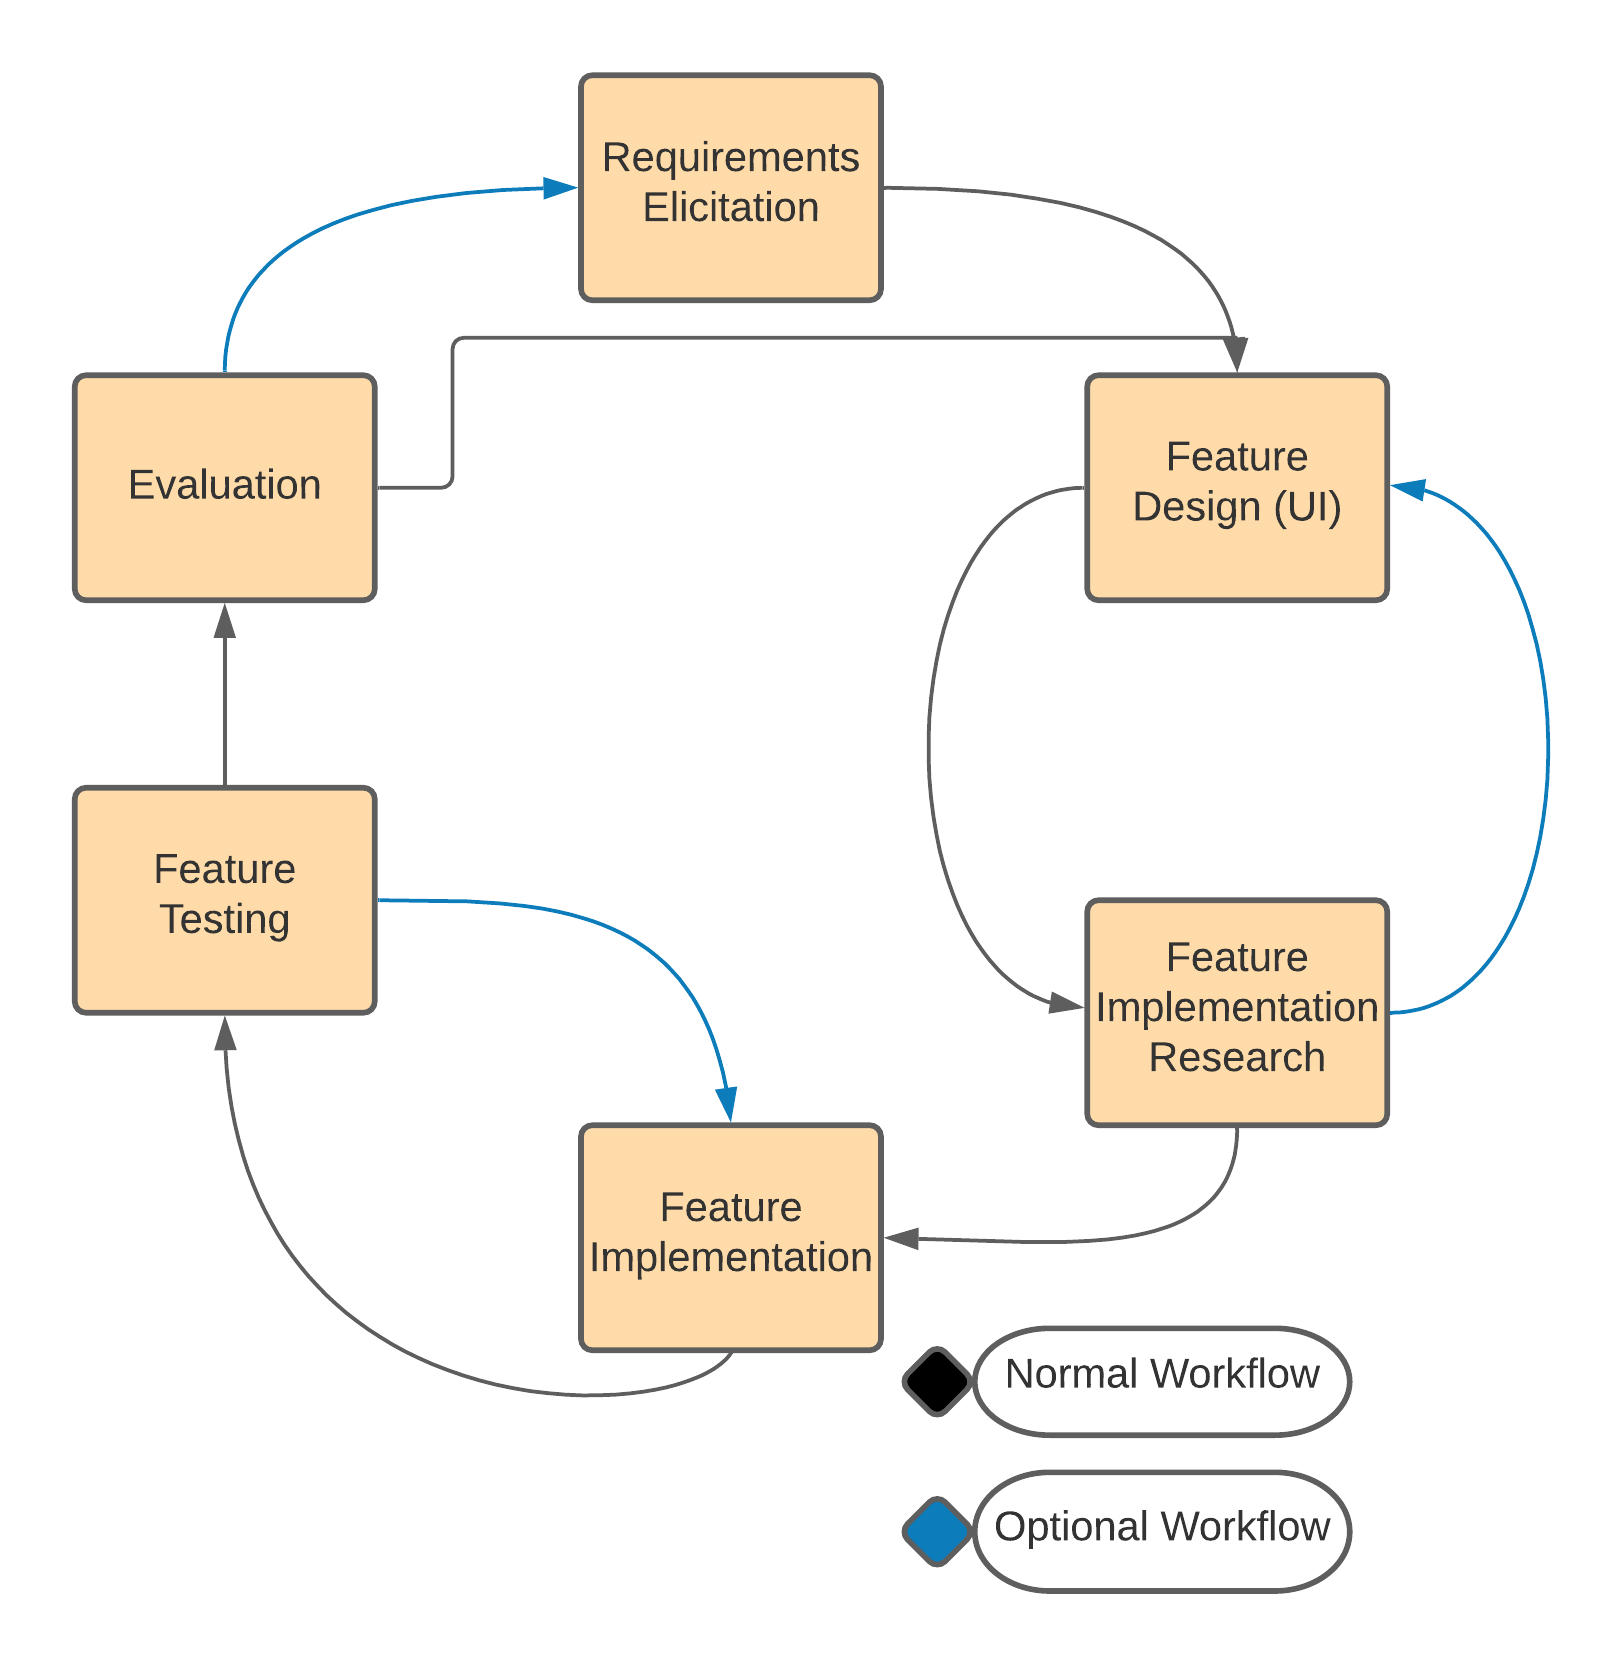
\includegraphics[scale=0.75]{Images/Project_Management_Methodology}
    \caption{Development Lifecycle}
    \label{fig:development lifecycle}
  \end{center}
\end{figure}
Throughout the project the focus of the workflow will shift as illustrated by the diagram below.

\begin{figure}
  \begin{center}
    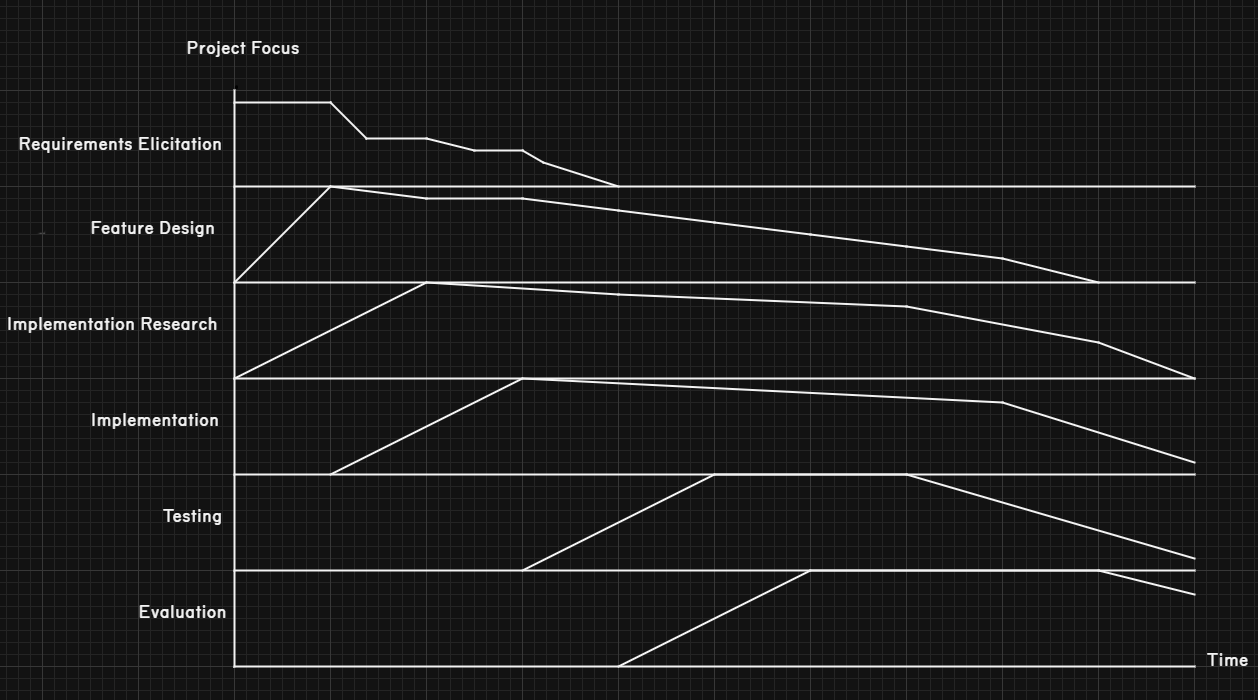
\includegraphics[scale=0.4]{Images/ProjectFocus2}
    \caption{Project Focus Over Time}
    \label{fig:project focus}
  \end{center}
\end{figure}
\section{Evaluation Design}
 (what method(s), used how, with what and how many participants?)

\section{Requirements Elicitation}
  How will requirements of the software be determined.

\section{Feature management}
  To track the creation and completion of features, a Kanban board will be used. This will include columns for 'To do', 'Doing' and 'Done'.

\section{Design Methods}
   \begin{itemize}
     \item Requirements Elicitation
     \begin{itemize}
       \item To better conceptualize the needs of the user. Use case diagrams and activity diagrams will be utilized.
     \end{itemize}
     \item User Interface
     \begin{itemize}
       \item Wireframes will be uitilized to establish interface element placement i.e. layout.
       \item More detailed mockups will be created when the earlier wireframes are constructed as prototypes and the concept is proved acheivable.
       \item A colour picker will be utilized to define the colour scheme.
       \item In later iterations of the design, once there is a functioning UI, usability will continue to be refined with the help of existing usability research, to guide the usage of font/colour/highlight on hover/font size etc.
       \item Additionally once a desktop friendly layout has been established, work will begin on optimizing a version for mobile.
     \end{itemize}
     \item Back-End
     \begin{itemize}
       \item UML will be used to show the overall design of the system through structural diagrams. These will show the interfaces of the classes and how they will interact with one another.
     \end{itemize}
   \end{itemize}

\section{Testing methods}

\section{Version control}
  I will be using Git and Github. This will allow the creation of branches to explore experimental parts of the soloution space without disrupting the progress of the main branch. If the experimental implementation is successfull it will be merged with the main branch. It also allows the development of features in paralel, with any conflicts in their implementation being resolved at the merge stage. The inclusion of a remote repository allows for work to continue on a seperate machine if nececarry and later be synced with the local main branch.
  \begin{figure}[H]
    \begin{center}
      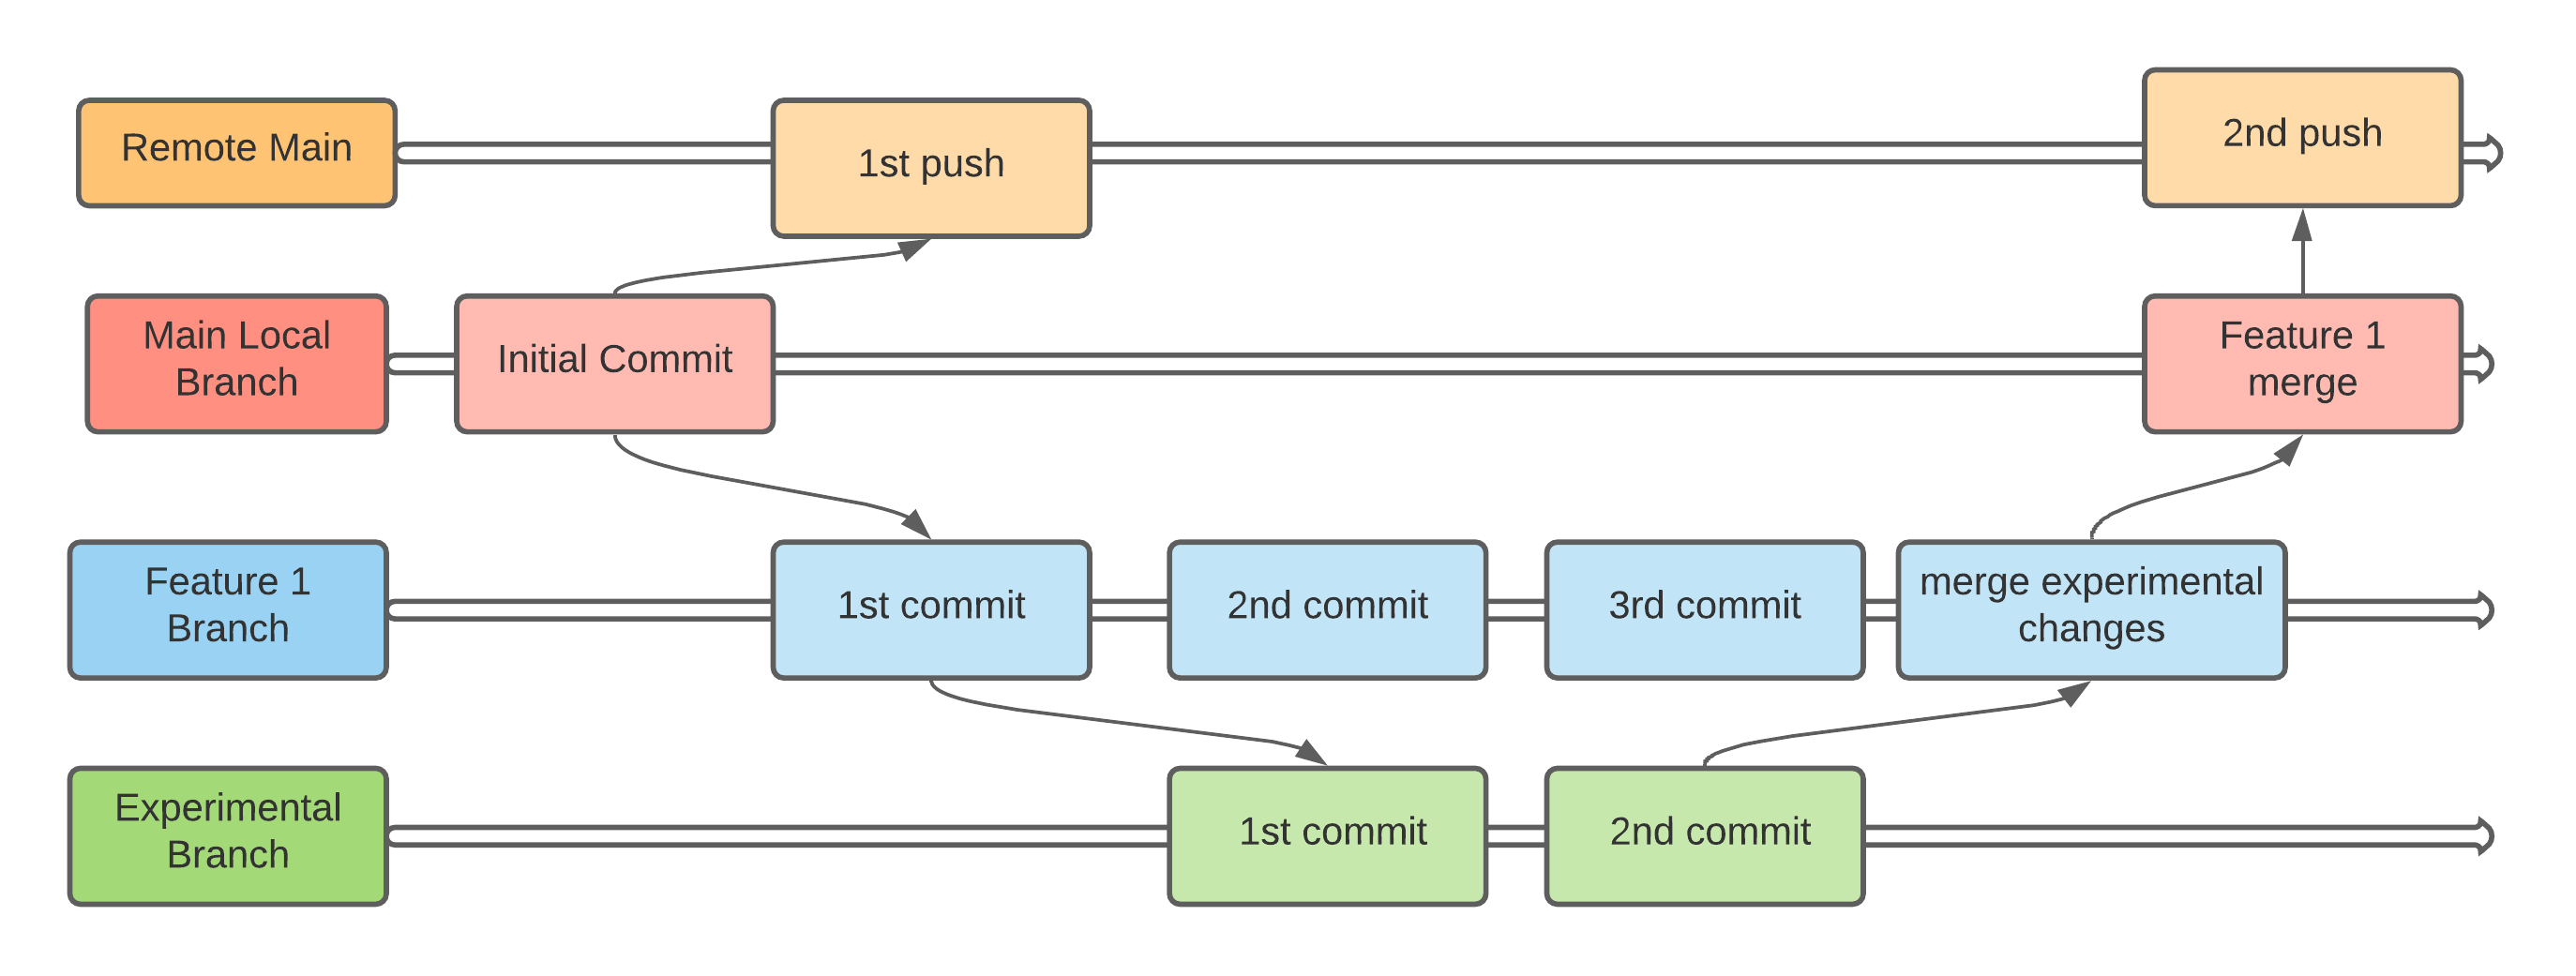
\includegraphics[scale=0.7]{Images/Git_Workflow_Diagram}
      \caption{Example Workflow To Highlight Branch Usage}
      \label{fig:Git Workflow}
    \end{center}
  \end{figure}

\section{Evaluation methods}
  The main method that will be utilized to determine the quality of the user interface will be the System Usability Scale (SUS) which can be seen here.
  The data will be collected via online questionare.
  % insert reference here
  Aditional metrics that focus on the evaluation of the CNN will be:
  \begin{itemize}
    \item Time to train the network on available hardware
    \begin{itemize}
      \item The constraint here being if the network cannot be trained on the available hardware in under sixteen hours. Purely for practical considerations.
    \end{itemize}
    \item Accuracy of CNN predictions. (which will be most effective when there are equal numbers of samples belonging to each class) $Accuracy = \frac{Correct Predicitons}{Total Predictions}$ Else if the samples are sqewed, the network could be a faliure at detecting a specific under-represented class, yet still score high accuracy.
    \item Precision. This is the number of correctly predicted images out of all predictions of that class. $Precision = \frac{Correctly Predicted for Class}{Total Predicted for Class}$ The network is precice for a class when the predictions it does make are correct. Precicion cannot be used in isolation due to the fact that the network can have a high precicion for a class but still fail to identify the majority of images for that class. Succeeding soley on the fact that the images it has classified are correct.
    \item Recall. Is the correct number of predictions for a class out of the number present of that class. $Recall = \frac{Correct Predicted for Class}{No. Present For Class}$
    This metric can also not be used in isolation due to the fact it does not take in to account the number of false positives. i.e. The number of images incorectly classified as the class in question. For example, if an image dataset contained three classes A, B, C, and the classfiier labeled all images A. The recall for A would be 100 percent.
    \item F1 score. This metric tries to find the balance between precision and recall and can be expressed as $F1 = 2 \times \frac{1}{\frac{1}{precicion} + \frac{1}{recall}}$
  \end{itemize}
\section{Initial Designs}
Firstly I have created a wireframe UI
  \begin{figure}[H]
    \begin{center}
      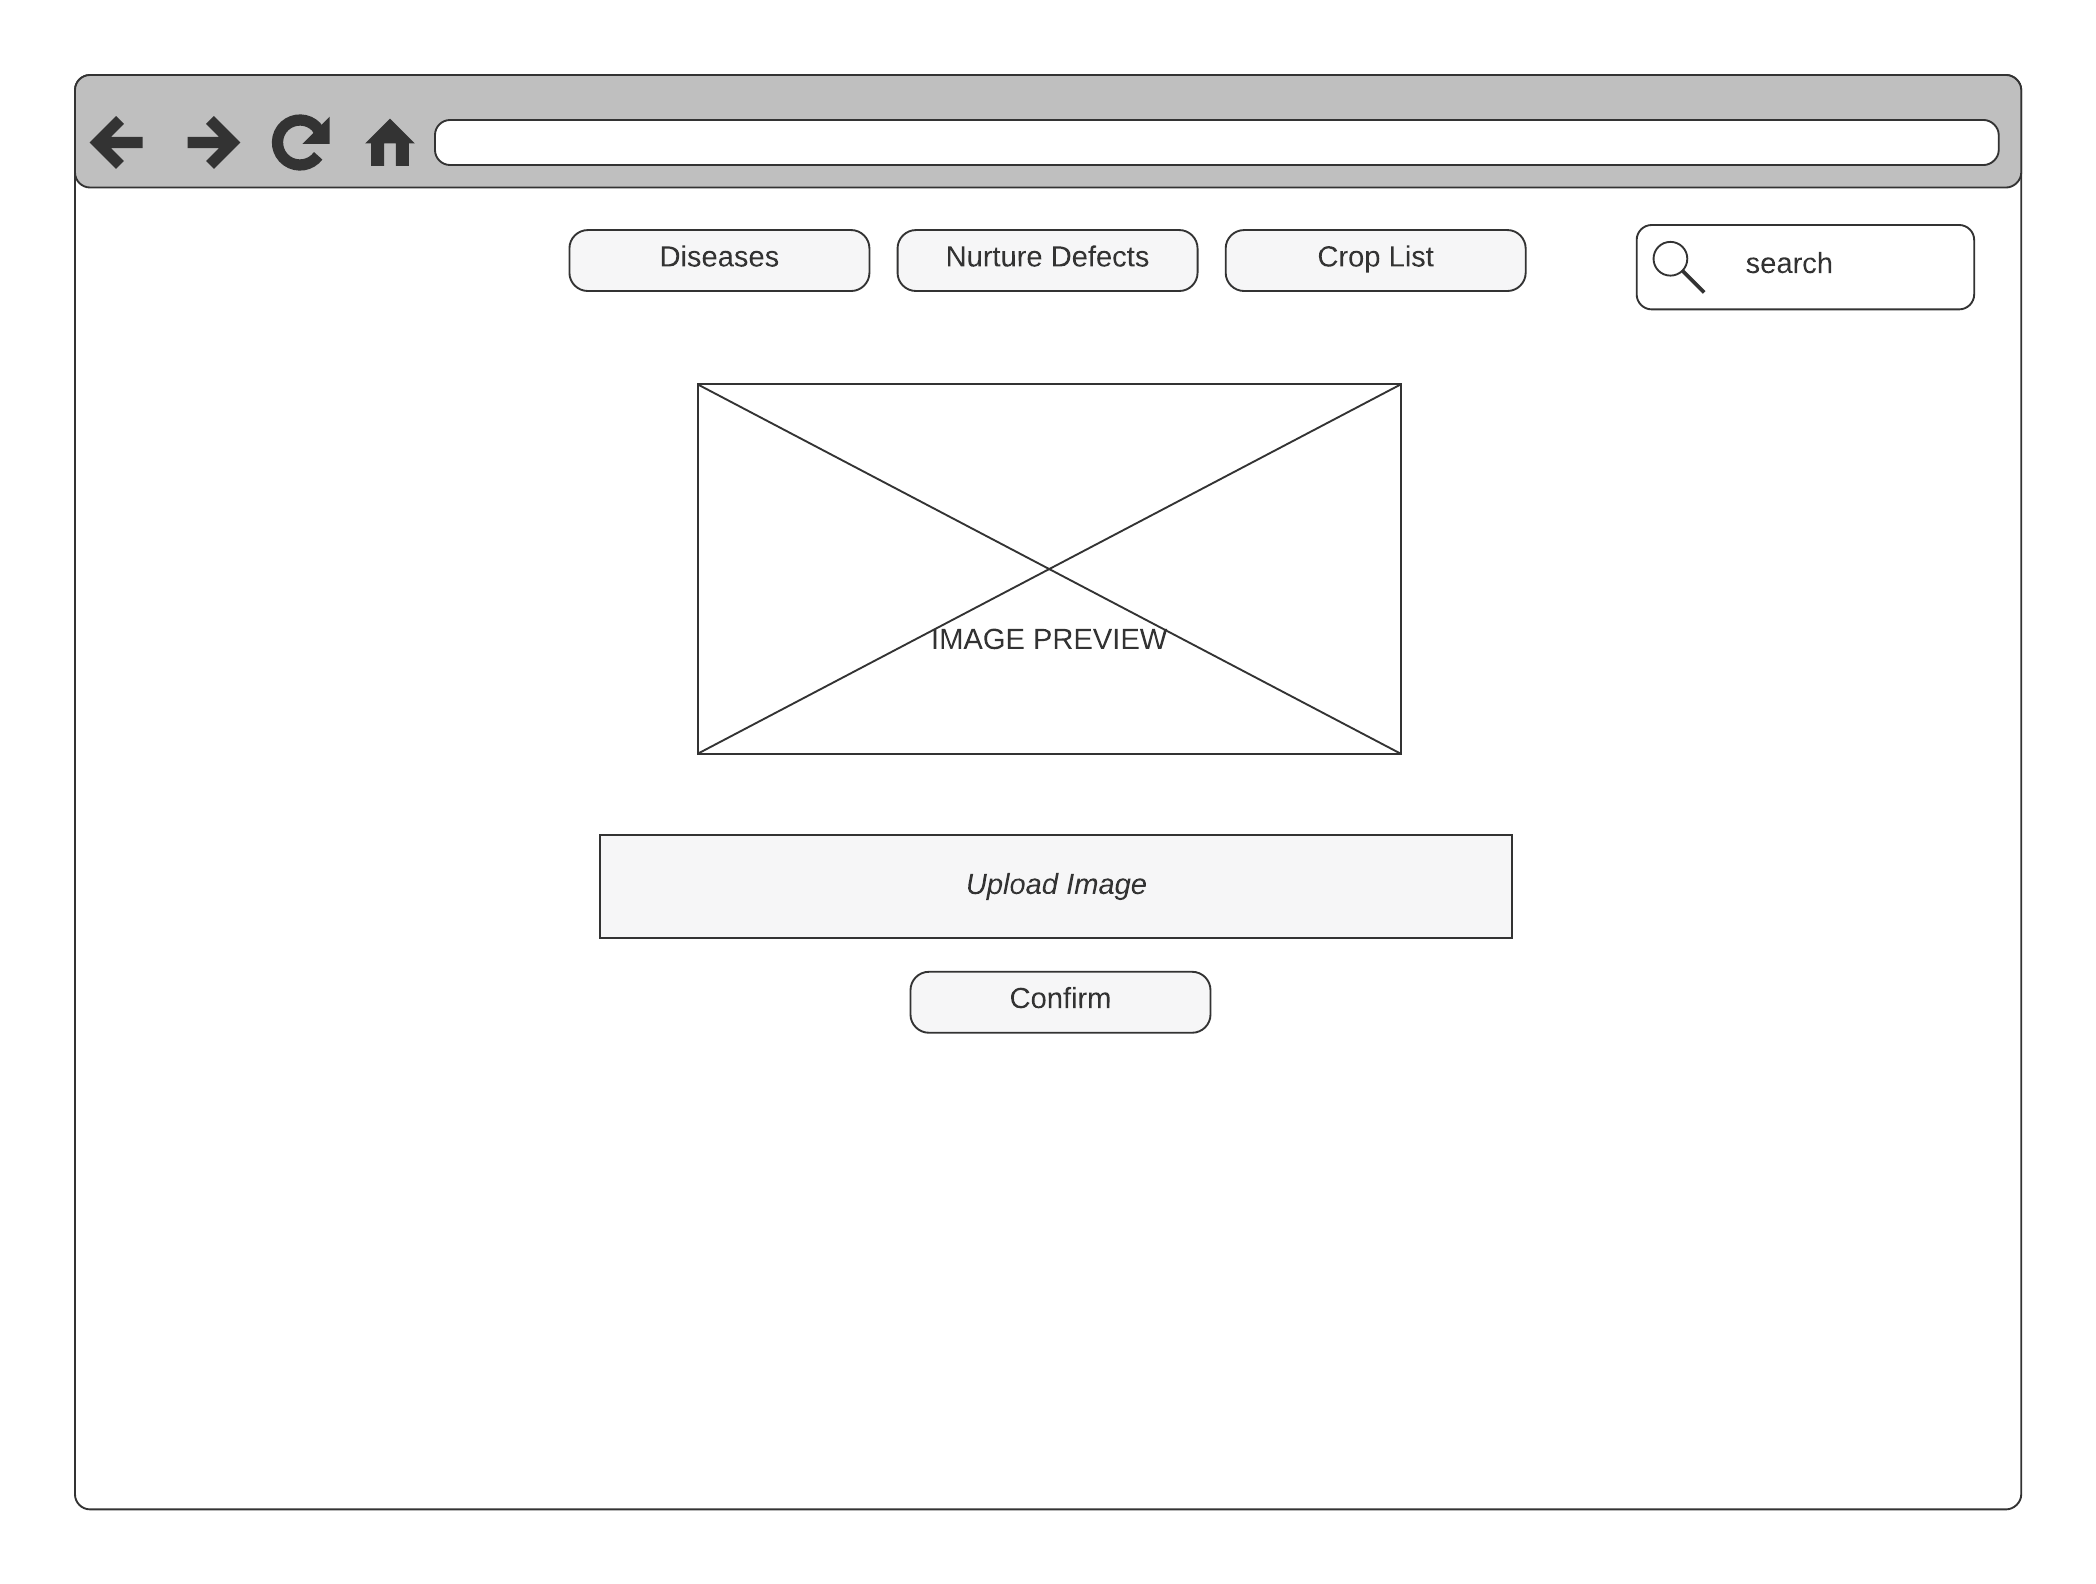
\includegraphics[scale=0.7]{Images/Home_Page_Wireframe}
      \caption{Homepage Wireframe}
      \label{fig:homepage_wireframe}
    \end{center}
  \end{figure}
  \begin{figure}[H]
    \begin{center}
      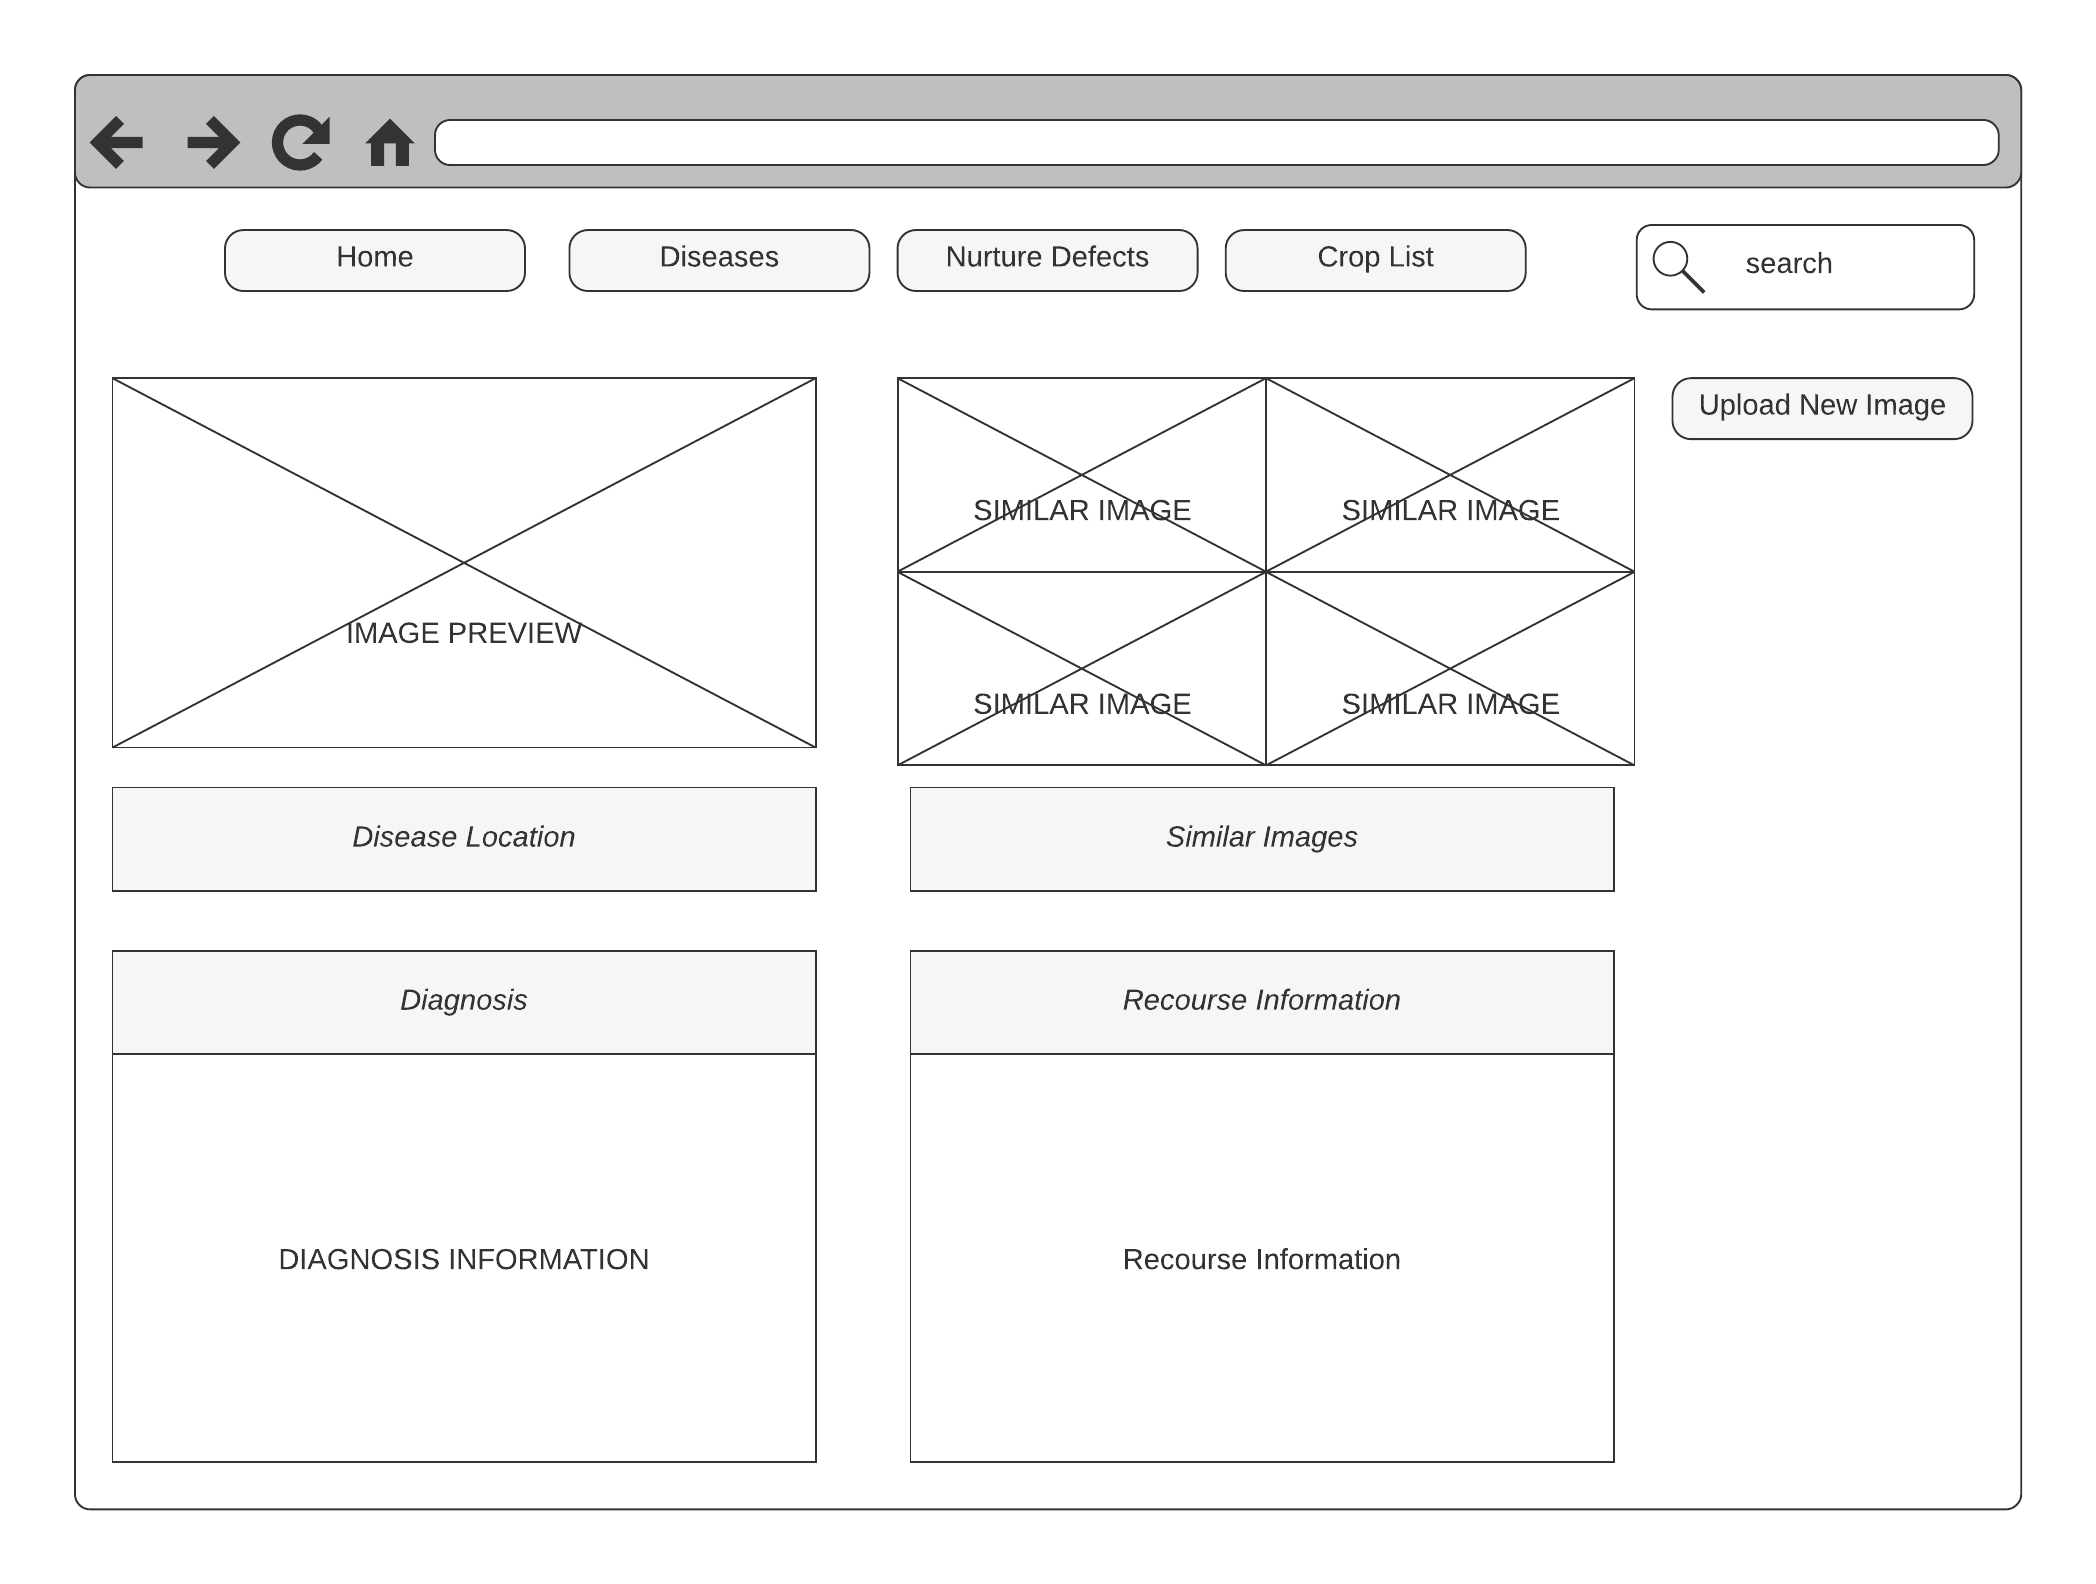
\includegraphics[scale=0.7]{Images/Defect_Information_Wireframe}
      \caption{Defect Information Wireframe}
      \label{fig:defect_wireframe}
    \end{center}
  \end{figure}
  \begin{figure}[H]
    \begin{center}
      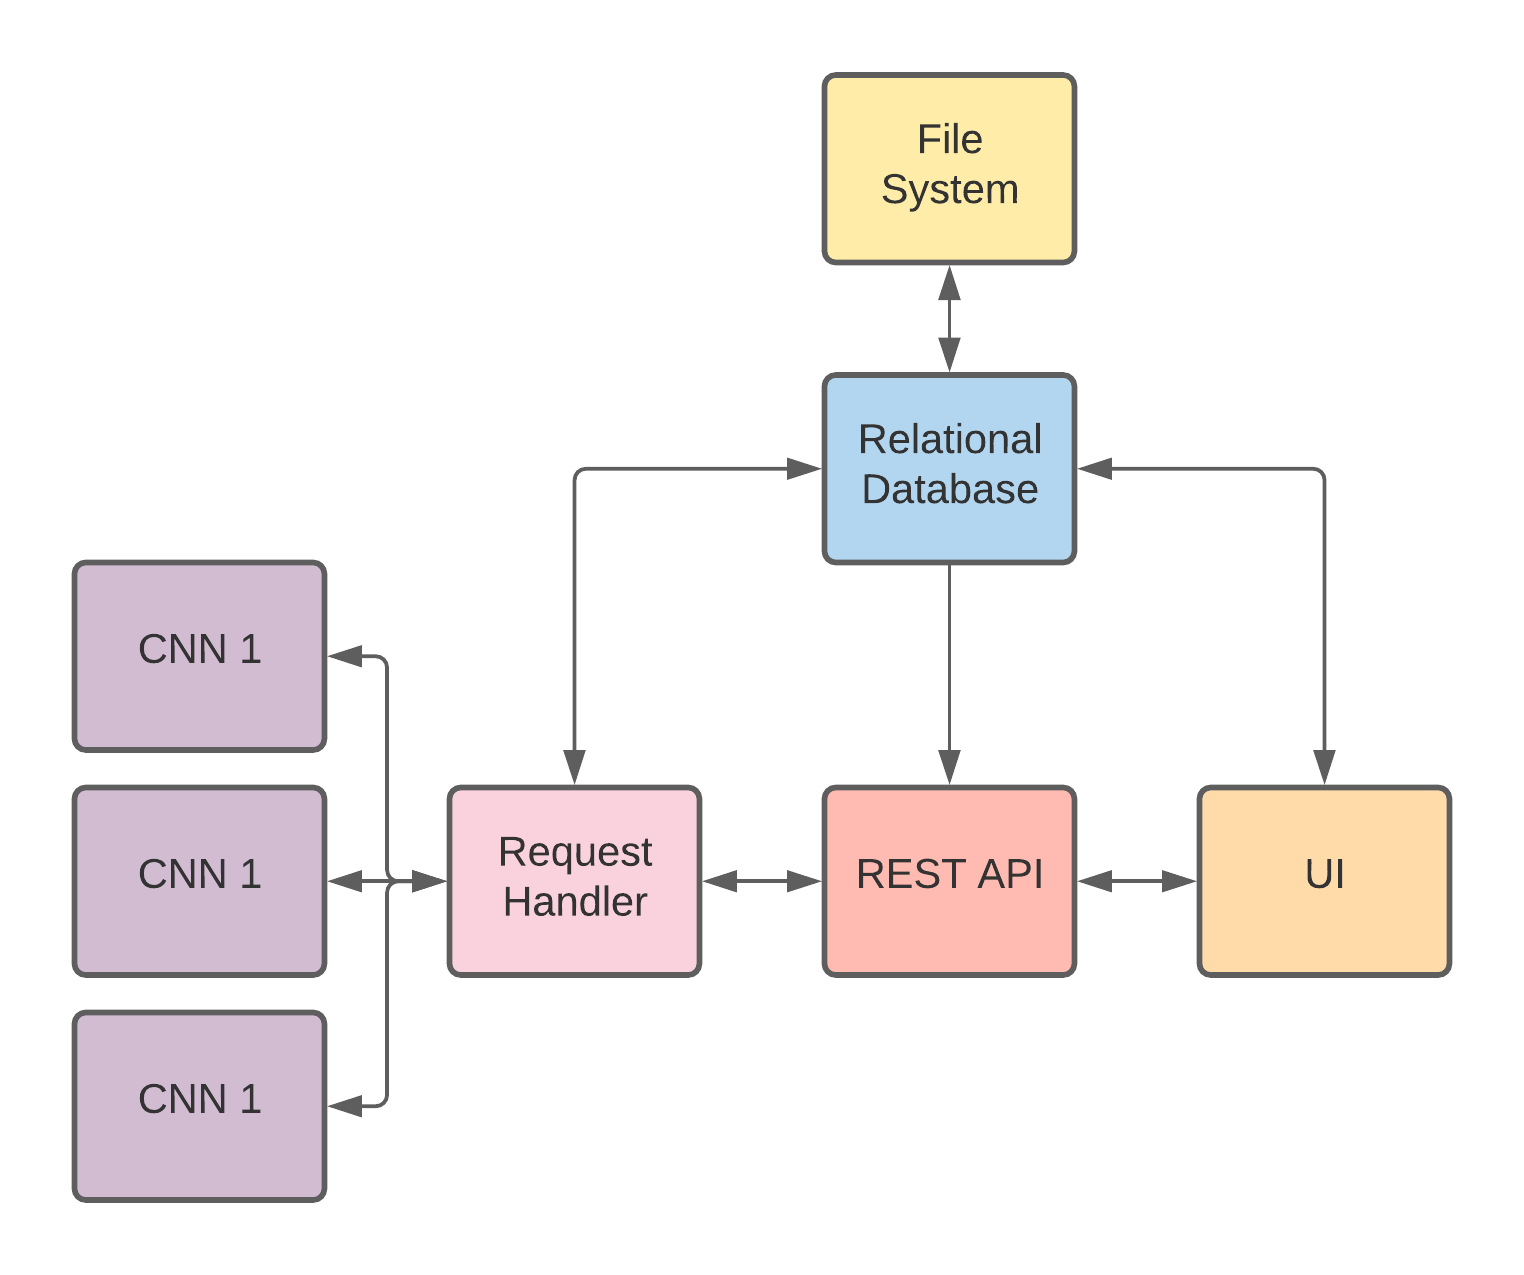
\includegraphics[scale=0.7]{Images/System_Overview_v1}
      \caption{System Overview}
      \label{fig:sys_overview}
    \end{center}
  \end{figure}
    \begin{figure}[H]
      \begin{center}
        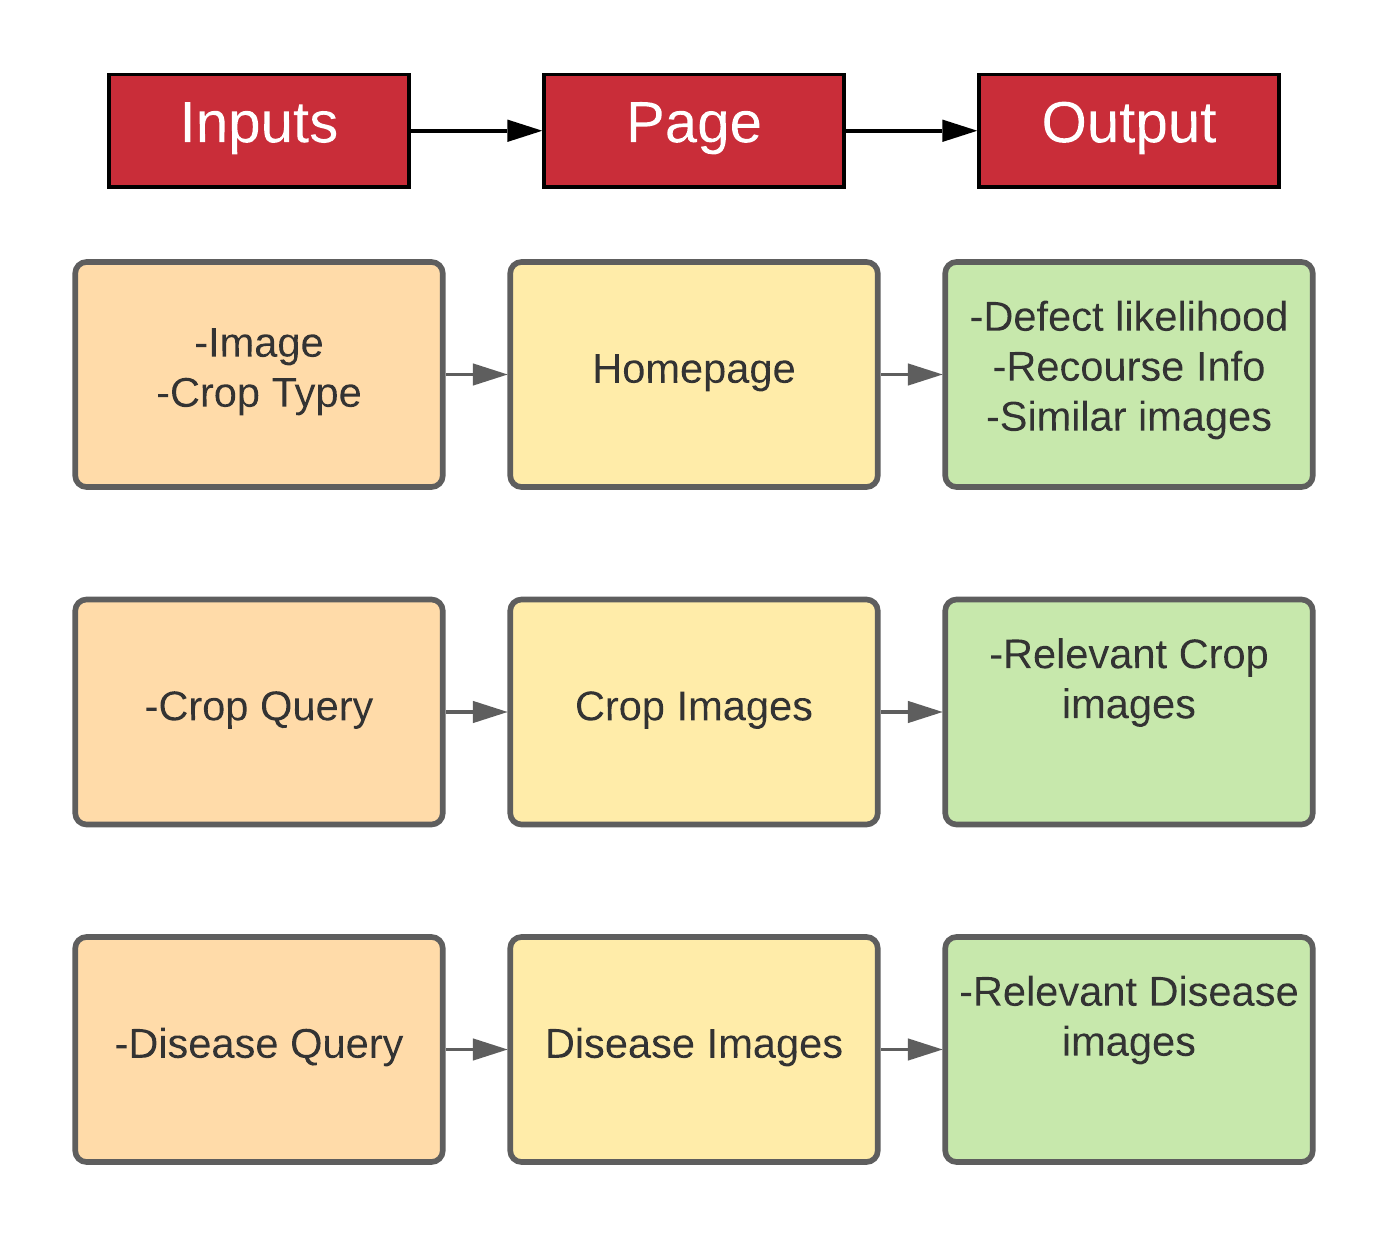
\includegraphics[scale=0.7]{Images/Input_Output_UI}
        \caption{Input/Output overview}
        \label{fig:input_output}
      \end{center}
    \end{figure}
    \end{figure}
      \begin{figure}[H]
        \begin{center}
          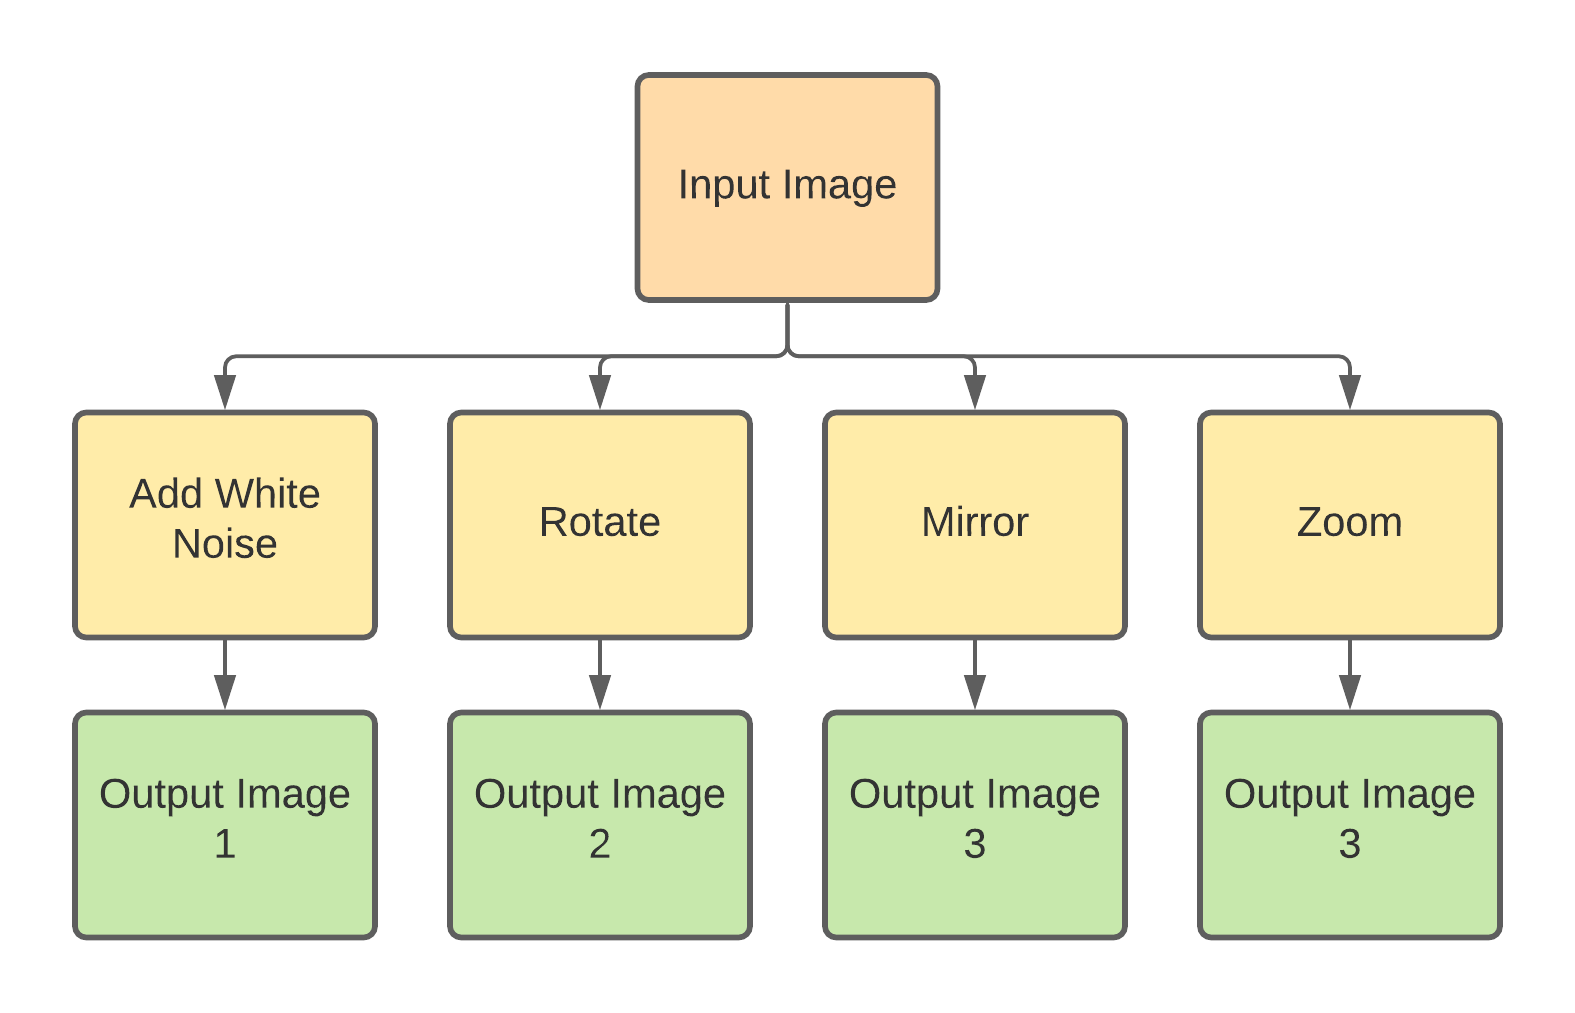
\includegraphics[scale=0.7]{Images/Data_Augmentation}
          \caption{Input/Data Augmentation Methods}
          \label{fig:data_augmentation}
        \end{center}
      \end{figure}

\section{Requirements}
  TEST TEXT
\section{Testing and Implementation details}

\section{Justification of Implementation Choices}
